%IMPORTS
\documentclass[a4paper, 11pt]{article}
\usepackage[utf8]{inputenc} 
\usepackage[T1]{fontenc}
\usepackage[catalan]{babel}
\usepackage{amsmath, amssymb, amsthm}
\usepackage[margin=1in]{geometry}
\usepackage{enumerate}
\usepackage{array}
\usepackage{graphicx}
\usepackage{wrapfig}
\usepackage{ragged2e} 
\usepackage{subfig}
\usepackage{caption}
\usepackage{subcaption}
\usepackage[dvipsnames]{xcolor}
%\usepackage[table]{xcolor}
\usepackage{float}
\usepackage{chngcntr}
\usepackage{ragged2e}
\usepackage{multirow}
\usepackage{vmargin}
\usepackage{hyperref}
\usepackage{url}
\usepackage{fancyhdr}
\usepackage{bigints}
\usepackage{listings}
\usepackage{xcolor,colortbl}
\usepackage{enumitem}
% \usepackage[english, spanish]{babel}
% \usepackage{slashbox}
\usepackage{diagbox}


\definecolor{navy}{rgb}{0,0,128}
\definecolor{codegreen}{rgb}{0,0.6,0}
\definecolor{codegray}{rgb}{0.5,0.5,0.5}
\definecolor{codepurple}{rgb}{0.58,0,0.82}
\definecolor{backcolour}{rgb}{0.95,0.95,0.92}
\definecolor{amaranth}{rgb}{0.9, 0.17, 0.31}
\definecolor{GRAY}{rgb}{0.75, 0.75, 0.75}


\lstdefinelanguage{Sage}[]{Python}
{morekeywords={False,sage,True},sensitive=true}
\lstset{
  frame=none,
  showtabs=False,
  showspaces=False,
  showstringspaces=False,
  commentstyle={\ttfamily\color{dgreencolor}},
  keywordstyle={\ttfamily\color{dbluecolor}\bfseries},
  stringstyle={\ttfamily\color{dgraycolor}\bfseries},
  language=Sage,
  basicstyle={\fontsize{10pt}{10pt}\ttfamily},
  aboveskip=0.3em,
  belowskip=0.1em,
  %numbers=left,
  numberstyle=\footnotesize
}
\definecolor{dblackcolor}{rgb}{0.0,0.0,0.0}
\definecolor{dbluecolor}{rgb}{0.01,0.02,0.7}
\definecolor{dgreencolor}{rgb}{0.2,0.4,0.0}
\definecolor{dgraycolor}{rgb}{0.30,0.3,0.30}
\newcommand{\dblue}{\color{dbluecolor}\bf}
\newcommand{\dred}{\color{dredcolor}\bf}
\newcommand{\dblack}{\color{dblackcolor}\bf}

\lstset{
morekeywords={var}
}
\lstset{
morekeywords={imag}
}
\lstset{
morekeywords={real}
}
\lstset{
morekeywords={contour\_plot}
}
\lstset{
morekeywords={streamline\_plot}
}
\lstset{
morekeywords={show}
}
\lstset{
morekeywords={plot\_vector\_field}
}

\setpapersize{A4}
\setmargins{2.5cm}     % margen izquierdo
{2.6cm}                % margen superior
{16.5cm}               % anchura del texto
{23.7cm}               % altura del texto
{10pt}                 % altura de los encabezados
{0cm}                  % espacio entre el texto y los encabezados
{0pt}                  % altura del pie de página
{1cm}                  % espacio entre el texto y el pie de página
\renewcommand{\baselinestretch}{1.5}

\begin{document}

\begin{titlepage}
    \centering
    {\bfseries\LARGE \hspace{2em} Universitat Autònoma de Barcelona\newline Facultat de Ciències\par}
    \vspace{2cm}
    {\hspace{-1em}
\includegraphics[width=0.4\textwidth]{logo.png}\par}
    \vspace{1cm}
    {\scshape\Huge Seminari 4: Transformada de Fourier\par} 
    \vspace{1cm}
    {\Large \itshape Autors: \par}
    {\Large  Gerard Lahuerta \& Ona Sánchez \& Andrea González \par}
    {\Large 1601350 --- 1601181 --- 1603921 \par}
    \vspace{1cm}
    {\Large 25 de Maig del 2022\par}
\end{titlepage}

\justifying

\newpage
\setcounter{page}{2}
\pagestyle{plain}
\tableofcontents
\cleardoublepage
\addcontentsline{}{chapter}{}
\newpage
\section{Exercicis per entregar}
\subsection{Exercici 5.6.7}
Provar l'igualtat de \textit{Plancherel}: $\sum_{j = 0}^{N-1} f[k]\overline{g[k]} = \frac{1}{N} \sum_{k = 0}^{N-1} \hat{f}[k] \overline{\hat{g}[k]}$
$$\sum_{k = 0}^{N-1} f[k]\overline{g[k]} = \left( \sum_{k = 0}^{N-1} \sum_{j = 0}^{N-1}\frac{1}{N} \hat{f}[k] e^{\frac{2\pi i j k}{N}} \cdot \sum_{j = 0}^{N-1} \frac{1}{N} \overline{\hat{g}[k] e^{\frac{2\pi i j k}{N}}}\right) = \frac{1}{N}  \sum_{k = 0}^{N-1} \hat{f}[k] e^{\frac{2\pi i j k}{N}} \overline{\hat{g}[k]} \cdot e^{\frac{-2\pi i j k}{N}} = \frac{1}{N} \sum_{k = 0}^{N-1} \hat{f}[k] \overline{\hat{g}[k]}$$
\textit{S'han utilitzat propietats en la demostració que són demostrades als exercicis extres, es  pot consultar a l'apartat \textcolor{blue}{\ref{extra}}}.
\subsection{Exercici 5.11.12}
Considereu un senyal amb les dades contingudes al fitxer \textbf{dades\_exer.csv} (es donen els valors $f[k]$). Estudieu el senyal (discret) i el seu espectre.

\begin{verbatim}
import csv
dadescsv=list(csv.reader(open("/home/gerard/Descargas/dades_exer.csv")) )
print(len(dadescsv))
\end{verbatim}
L'output obtingut i que serveix per comprovar que les dades han sigut extretes de forma correcte és:
\begin{verbatim}
    128
\end{verbatim}
A continuació, una vegada confirmada l'extracció correcte de les dades, procedim a analitzar el senyal:
\begin{verbatim}
dades_llista=[RR(dadescsv[j][0]) for j in range(len(dadescsv))]
long=len(dades_llista)
T=40
fft_dades=FFT(long)
for j in range(long):
    fft_dades[j]=dades_llista[j]
fft_dades.forward_transform()
fft_dades_freq=[[0,0] for k in range(long/2)]
for j in range(long/2):
    fft_dades_freq[j][0]=j/T
    fft_dades_freq[j][1]= abs(vector(fft_dades[j]))/long

dibS=list_plot(fft_dades_freq,plotjoined=True,axes_labels=('Freq. angular', 'Amplitud'),
                color = 'red')
dades_temps=[[0,0] for k in range(long)]
for j in range(long):
    dades_temps[j][0]=j*T/long
    dades_temps[j][1]= dades_llista[j]
dibT=list_plot(dades_temps,plotjoined=True,axes_labels=('Temps', 'Senyal'))
Dib=graphics_array([dibT,dibS])
show(Dib,figsize=[12, 5])
\end{verbatim}
Del codi mostrat, s'obté el següent output, gràfic de l'espectre del senyal:
\begin{figure}[h]
    \centering
    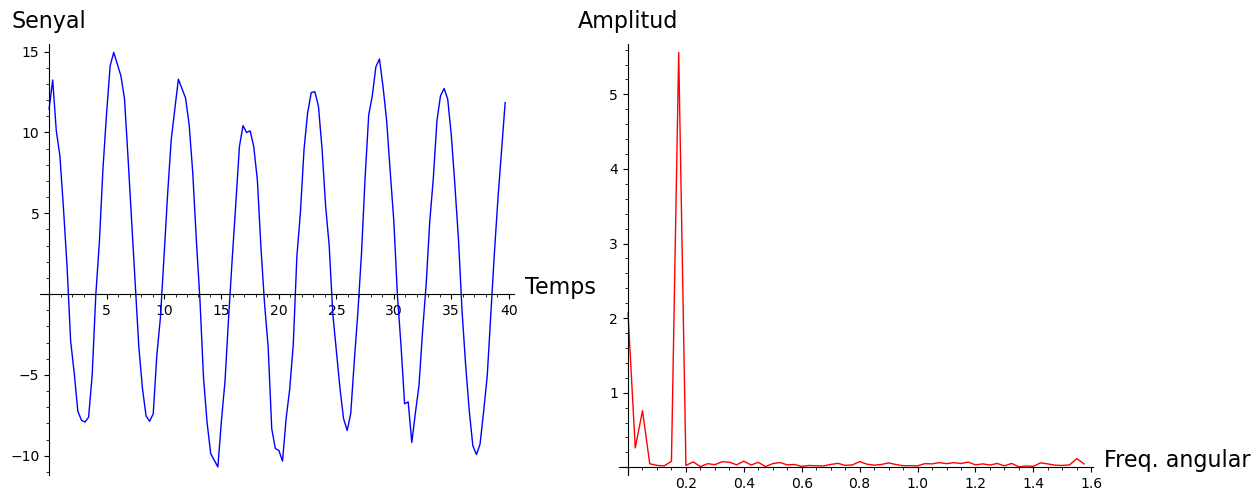
\includegraphics[width=1\textwidth]{12.png}
    \caption{Output del programa}
    \label{fig:my_label}
\end{figure}\\
És pot observar fàcilment com el senyal no és del tot clar (hi existeixen interferències/soroll) pel que les petites "deformitats" \hspace{0.0625 em} de la gràfica afecten a l'anàlisis de les freqüències.\\
Podem deduïr que existeix una presència notoria de 3 pics diferents (situats a $0, 0.05$ i $0.2$).\\
De totes les frequències rellevants, la més important i la que resalta davant de totes és la situada a $0.2$.\\
Com que la diferència d'amplituts entre la més notoria i les altres és molt gran, podem asumir que la resta de freqüències són part del soroll; és a dir, concluïm que la freqüència del senyal es situa a $0.2$ i la resta de freqüències que apareixen a l'espectre es tracten de "soroll"\hspace{0.0625 em} de fons.
\newpage
\section{Exercicis extres}\label{extra}
\subsection{Exercici 5.1.1}
Proveu que $\hat{f}[k+N] = \hat{f}[k]$.\\
$$ \hat{f}[k+N] = \sum_{j = 0}^{N-1} \left( f[j+N]\cdot e^{\frac{−2\pi i j k}{N}}\right) = \sum_{j = 0}^{N-1} \left( f[j]\cdot e^{\frac{−2\pi i j k}{N}}\right) = \hat{f}[k] \Longrightarrow \hat{f}[k+N] = \hat{f}[k]$$
\subsection{Exercici 5.1.2}
Calcular $\hat{f}[k]$ si $N=4$ i $f[0]=f[1]=0$ i $f[2]=f[3]=1$.\\
$$e(-i\pi k) + e(-\frac{3}{2}i\pi k)$$
\subsection{Exercici 5.1.3}
Proveu les següents propietats
\begin{itemize}
    \item Linealitat. $(\alpha f + \beta g)^ = \alpha \hat{f} + \beta \hat{g}$.\\
     $$ (\alpha f + \beta g)\hat{} = \sum_{j = 0}^{N-1} \left( (\alpha f + \beta g)\cdot e^{\frac{−2\pi i j k}{N}}\right) = \sum_{j = 0}^{N-1} \left( \alpha f \cdot e^{\frac{−2\pi i j k}{N}} + \beta g \cdot e^{\frac{−2\pi i j k}{N}}\right) = $$ $$=\sum_{j = 0}^{N-1} \left( \alpha f \cdot e^{\frac{−2\pi i j k}{N}} \right) + \sum_{j = 0}^{N-1} \left( \beta g \cdot e^{\frac{−2\pi i j k}{N}}\right) = $$ $$ = \alpha \sum_{j = 0}^{N-1} \left( f \cdot e^{\frac{−2\pi i j k}{N}} \right) + \beta \sum_{j = 0}^{N-1} \left( g \cdot e^{\frac{−2\pi i j k}{N}}\right) = \alpha \hat{f} + \beta \hat{g}$$
    \item Translació temporal. Si $g[k] = f[k-n]$ llavors $\hat{g}[k] = e^{-2\pi ikn/N} \hat{f}[k]$.\\
    $$ \hat{g}[k-n] = \sum_{j = 0}^{N-1} \left( f[j-n]\cdot e^{\frac{−2\pi i (j-n) k}{N}} \cdot e^{\frac{-2\pi i j n k}{N}}\right) =  e^{\frac{2\pi i n k}{N}} \sum_{j = 0}^{N-1} \left( f[j-n]\cdot e^{\frac{−2\pi i (j-n) k}{N}}\right) = e^{\frac{2\pi i n k}{N}} \cdot \hat{f}[k] $$
    \item Translació freqüencial. Si $g[k]$ = $f[k]e^{2\pi ikn/N}$ llavors $\hat{g}[k] = \hat{f}[k-n]$.\\
    $$ \hat{g}[k] = e^{\frac{2\pi i n k}{N}} \sum_{j = 0}^{N-1} \left( f[j]\cdot e^{\frac{−2\pi i j k}{N}}\right) = \sum_{j = 0}^{N-1} \left( f[j]\cdot e^{\frac{−2\pi i j k}{N}} \cdot e^{\frac{2\pi i n k}{N}}\right) = $$ $$=\sum_{j = 0}^{N-1} \left( f[j]\cdot e^{\frac{−2\pi i j k}{N}} \cdot e^{\frac{-2\pi i (-n) k}{N}}\right) = \sum_{j = 0}^{N-1} \left( f[j]\cdot e^{\frac{−2\pi i (j-n) k}{N}}\right) = \sum_{j = 0}^{N-1} \left( f[j-n]\cdot e^{\frac{−2\pi i (j-n) k}{N}}\right) = \hat{f}[k-n]$$
    \item Modulació. Si $g[k] = f[k]cos2\pi kn/N$ llavors $\hat{g}[k] = \frac{1}{2}(\hat{f}[k-n] + \hat{f}[k+n])$.\\
    $$ \hat{g}[k] = \sum_{j = 0}^{N-1} \left( f[j]\cdot \cos(\frac{2\pi k n}{N}) \right) = \sum_{j = 0}^{N-1} \left( f[j]\cdot \frac{1}{2}\left( e^{\frac{2\pi k n}{N}i} + e^{-\frac{2\pi k n}{N}i} \right) \right) = $$ $$=\frac{1}{2} \left( \sum_{j = 0}^{N-1} \left( f[j]\cdot e^{\frac{2\pi k n}{N}i} \right) + \sum_{j = 0}^{N-1} \left( f[j]\cdot e^{-\frac{2\pi k n}{N}i} \right) \right) = \frac{1}{2} \left( \hat{f}[k-n] + \hat{f}[k+n] \right)$$
\end{itemize}

\subsection{Exercici 5.5.6}
Provar que quan $f[k] = f(kT/N)$ llavors $c_j = \frac{1}{N} \hat{f}[j]$.\\
$$ p(x_k) = f(x_k) \Longleftrightarrow c_j \cdot e^{\frac{2\pi ijx}{T}} = \frac{1}{N} \hat{f}(jN/T) \cdot e^{\frac{2\pi ijkN}{TN}} \Longrightarrow c_j = \frac{1}{N} \hat{f}(jN/T) = \frac{1}{N} \hat{f}[j] \Longrightarrow c_j = \frac{1}{N} \hat{f}[j] $$
\subsection{Exercici 5.5.8}
Deduir que $\sum_{j = 0}^{N-1} |f[k]|^2 = \frac{1}{N} \sum_{j = 0}^{N-1} |\hat{f}[k]|^2$.
$$ \sum_{j = 0}^{N-1} |f[k]|^2 = \sum_{j = 0}^{N-1} f[k]\overline{f[k]} = \frac{1}{N} \sum_{j = 0}^{N-1} \hat{f}[k] \overline{\hat{f}[k]} = \frac{1}{N} \sum_{j = 0}^{N-1} |\hat{f}[k]|^2 $$
\subsection{Exercici 5.5.9}
Provar que $(f*g)\hat{}[k] = \hat{f}[k] \cdot \hat{g}[k] $
$$ (f*g)\hat{}[k] = \sum_{j = 0}^{N-1} (f*g)[k] (w^k)^j = \sum_{j = 0}^{N-1} \left( \sum_{q = 0}^{N-1} f[q]g[j-q] \right) (w^k)^j = \sum_{j = 0}^{N-1} \left( \sum_{q = 0}^{N-1} f[q]g[j-q] \right) w^{kj} =$$ $$= \sum_{j = 0}^{N-1} \sum_{q = 0}^{N-1} f[q]g[j-q] w^{kq} w^{k(j-q)} = \hat{f}[k] \cdot \hat{g}[k] $$
\newpage
\subsection{Exercici 5.11.11}
Tenim un senyal de la forma $f(t) = \frac{a_0}{2} + \sum_{k=1}^m (a_n cos(2\pi kx/T) + b_n sin(2\pi kx/T))$.\\
El gràfic del senyal s'ha realitzat amb el codi:
\small
\begin{verbatim}
    var('x')
    m = 10
    T = 100
    a0 = 1
    f = 0
    for k in range(1,m):
        f += 2*k*cos(2*pi*k*x/T)+k*sin(2*pi*k*x/T)
    N = 2**8
    plot(f, (x,-30,100))
\end{verbatim}
Que dona el següent senyal:
\begin{figure}[h]
\centering
 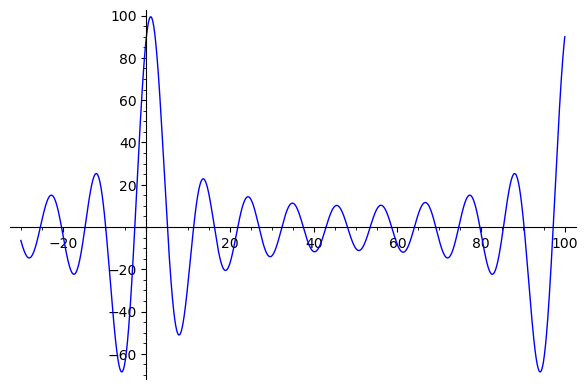
\includegraphics[width=0.5\textwidth]{meter1.png}
\end{figure}\\
S'ha generat una mostra $M = [f[0], f[1], ..., f[N-1]]$ de manera que $f[k]=f(k\cdot T/N) +$ soroll Gaussià.\\
S'ha generat amb el codi:
\begin{verbatim}
    data = []
    c = 3
    mean = 0
    sd = 10
    for i in range(0,2**7):
        res = [i,f(i*T/(2**7)).n()+c*gauss(mean,sd)]
        data.append(res)
    show(data)
\end{verbatim}
Les mostres generades son: 
$$[[0,78.8850326657057],[1,121.961528341471],[2,104.753021560335], ..., $$ $$ ..., [125,26.5845519022956],[126,30.9520577591478],[127,55.7335597110999]] $$
El dibuix de la mostra del senyal donat per M s'ha generat amb el codi:
\begin{verbatim}
    list_plot(data,plotjoined=True,axes_labels=('Temps', 'Senyal'))
\end{verbatim}\\
Que genera el dibuix:
\begin{figure}[h]
\centering
 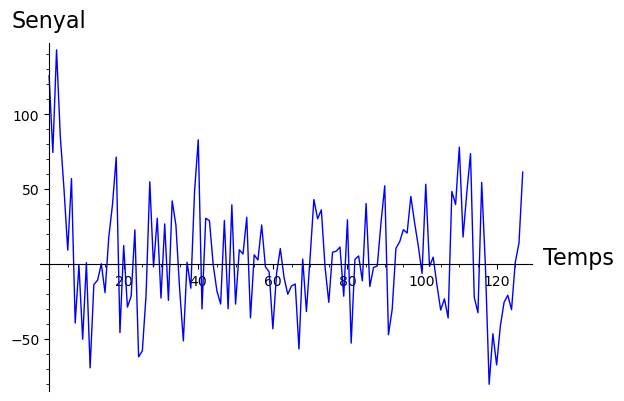
\includegraphics[width=0.5\textwidth]{meter2.png}
\end{figure}\\
S'ha fet el dibuix de l'amplitud sense soroll:
\begin{verbatim}
    long = len(data)
    fft_dades=FFT(long)
    
    for j in range(long):
        fft_dades[j]=data[j][1]
    fft_dades.forward_transform()    
        
    fft_funcio = FFT(N)
    for t in range(N):
        fft_funcio[t] = f(i*2*pi/(2**7))
    fft_funcio.forward_transform()
    
    
    fft_dades_freq=[[0,0] for k in range(long/2)]
    for j in range(long/2):
        fft_dades_freq[j][0]=j/T
        fft_dades_freq[j][1]= abs(vector(fft_dades[j]))/long
    
    fft_funcio_freq=[[0,0] for k in range(N/2)]
    for j in range(N/2):
        fft_funcio_freq[j][0]=j/T
        fft_funcio_freq[j][1]= abs(vector(fft_funcio[j]))/N
        
    list_plot(fft_funcio_freq,plotjoined=True, axes_labels=('Freq. angular', 'Amplitud'),
    color='red')
\end{verbatim}
\begin{figure}[h]
\centering
 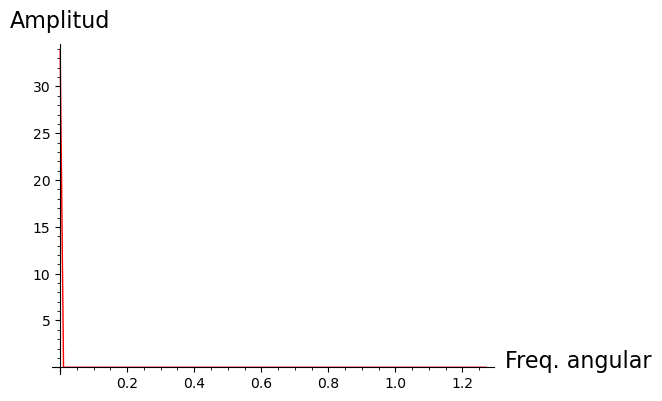
\includegraphics[width=0.5\textwidth]{meter3.png}
\end{figure}\\
Amb soroll:
\begin{verbatim}
    list_plot(fft_dades_freq,plotjoined=True,axes_labels=('Freq. angular', 'Amplitud'))
\end{verbatim}
\begin{figure}[h]
\centering
 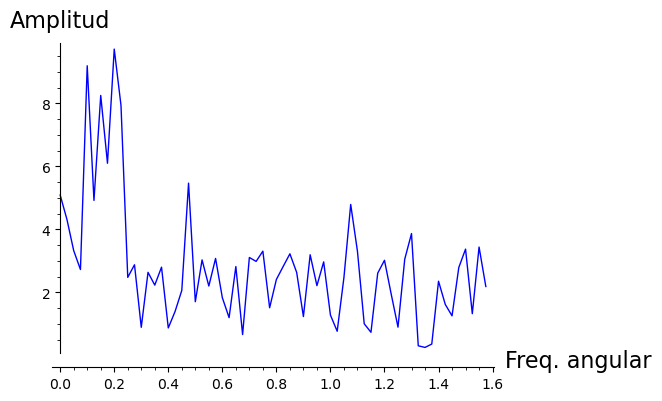
\includegraphics[width=0.5\textwidth]{11.png}
\end{figure}\\
\end{document}
